\documentclass{standalone}
\usepackage{tikz}
\usetikzlibrary{patterns, positioning}

\begin{document}
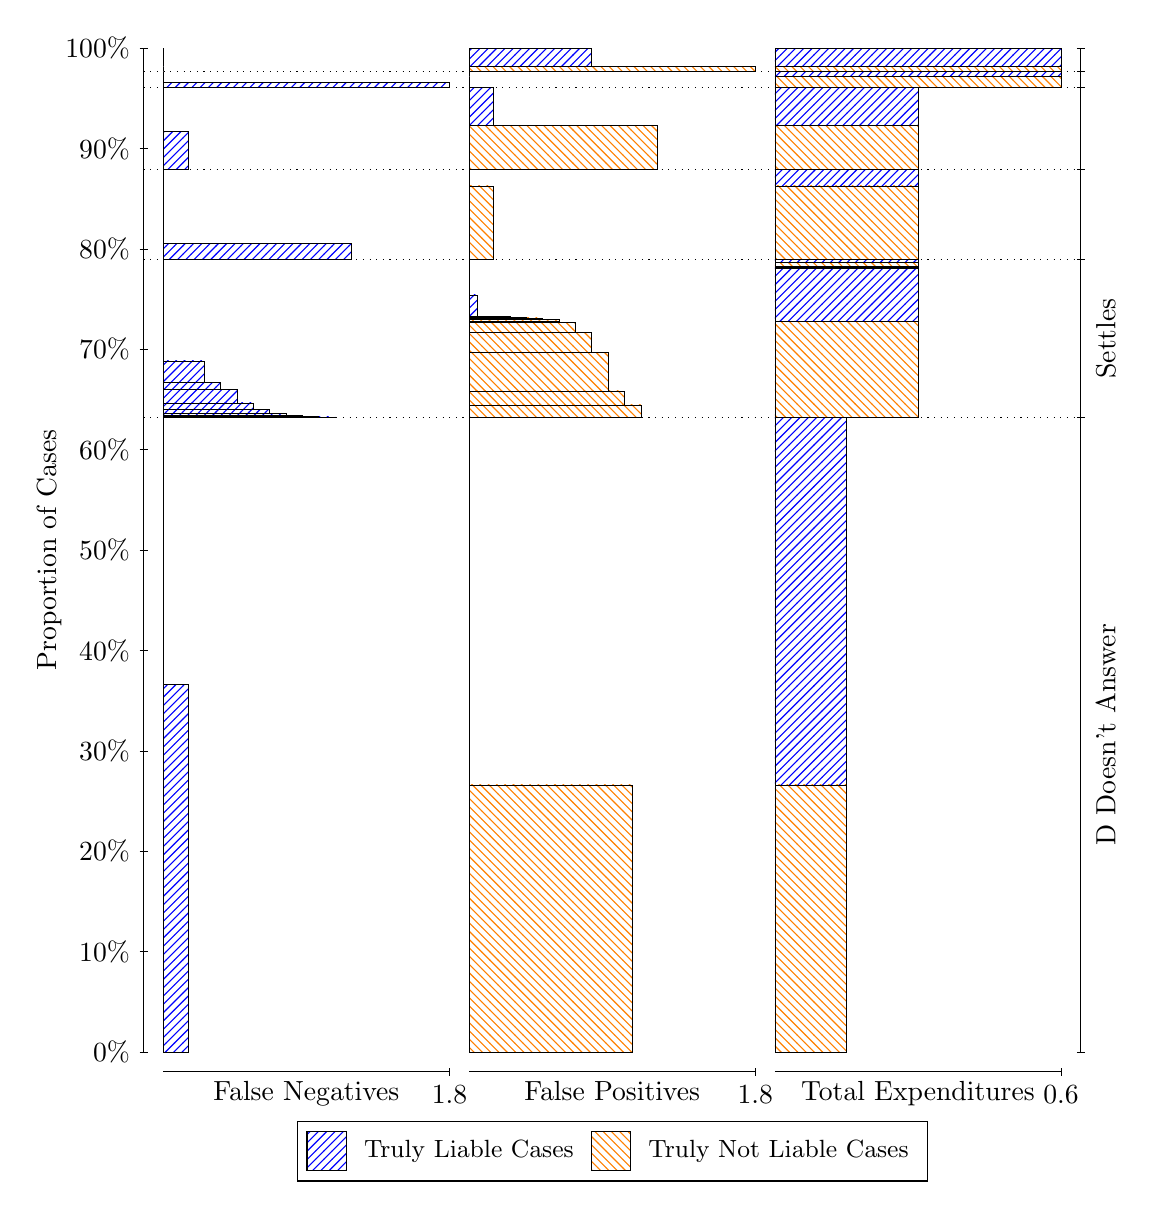
\begin{tikzpicture}
\draw[black, very thin] (1.5,1.75) -- (1.5,14.5);
\node[rotate=90, anchor=center] at (0.3, 8.125) {Proportion of Cases};
\draw[black, very thin] (1.45,1.75) -- (1.55,1.75);
\node[anchor=east] at (1.45, 1.75) {0\%};
\draw[black, very thin] (1.45,3.025) -- (1.55,3.025);
\node[anchor=east] at (1.45, 3.025) {10\%};
\draw[black, very thin] (1.45,4.3) -- (1.55,4.3);
\node[anchor=east] at (1.45, 4.3) {20\%};
\draw[black, very thin] (1.45,5.575) -- (1.55,5.575);
\node[anchor=east] at (1.45, 5.575) {30\%};
\draw[black, very thin] (1.45,6.85) -- (1.55,6.85);
\node[anchor=east] at (1.45, 6.85) {40\%};
\draw[black, very thin] (1.45,8.125) -- (1.55,8.125);
\node[anchor=east] at (1.45, 8.125) {50\%};
\draw[black, very thin] (1.45,9.4) -- (1.55,9.4);
\node[anchor=east] at (1.45, 9.4) {60\%};
\draw[black, very thin] (1.45,10.675) -- (1.55,10.675);
\node[anchor=east] at (1.45, 10.675) {70\%};
\draw[black, very thin] (1.45,11.95) -- (1.55,11.95);
\node[anchor=east] at (1.45, 11.95) {80\%};
\draw[black, very thin] (1.45,13.225) -- (1.55,13.225);
\node[anchor=east] at (1.45, 13.225) {90\%};
\draw[black, very thin] (1.45,14.5) -- (1.55,14.5);
\node[anchor=east] at (1.45, 14.5) {100\%};

\draw[black, very thin] (13.4,1.75) -- (13.4,14.5);
\draw[black, very thin] (13.35,1.75) -- (13.45,1.75);
\node[anchor=west] at (13.35, 1.75) {};
\draw[black, very thin] (13.35,9.8072) -- (13.45,9.8072);
\node[anchor=west] at (13.35, 9.8072) {};
\draw[black, very thin] (13.35,11.816) -- (13.45,11.816);
\node[anchor=west] at (13.35, 11.816) {};
\draw[black, very thin] (13.35,12.954) -- (13.45,12.954);
\node[anchor=west] at (13.35, 12.954) {};
\draw[black, very thin] (13.35,14) -- (13.45,14);
\node[anchor=west] at (13.35, 14) {};
\draw[black, very thin] (13.35,14.204) -- (13.45,14.204);
\node[anchor=west] at (13.35, 14.204) {};
\draw[black, very thin] (13.35,14.5) -- (13.45,14.5);
\node[anchor=west] at (13.35, 14.5) {};

\draw[black, very thin, pattern color=blue, pattern=north east lines] (1.75,1.75) rectangle (2.0614,6.4162);
\draw[black, very thin, pattern color=orange, pattern=north west lines] (1.75,6.4162) rectangle (1.75,9.8072);
\draw[black, very thin, pattern color=blue, pattern=north east lines] (1.75,9.8072) rectangle (3.93,9.8147);
\draw[black, very thin, pattern color=blue, pattern=north east lines] (1.75,9.8147) rectangle (3.7224,9.822);
\draw[black, very thin, pattern color=blue, pattern=north east lines] (1.75,9.822) rectangle (3.5148,9.8363);
\draw[black, very thin, pattern color=blue, pattern=north east lines] (1.75,9.8363) rectangle (3.3071,9.8582);
\draw[black, very thin, pattern color=blue, pattern=north east lines] (1.75,9.8582) rectangle (3.0995,9.9136);
\draw[black, very thin, pattern color=blue, pattern=north east lines] (1.75,9.9136) rectangle (2.8919,9.992);
\draw[black, very thin, pattern color=blue, pattern=north east lines] (1.75,9.992) rectangle (2.6843,10.165);
\draw[black, very thin, pattern color=blue, pattern=north east lines] (1.75,10.165) rectangle (2.4767,10.258);
\draw[black, very thin, pattern color=blue, pattern=north east lines] (1.75,10.258) rectangle (2.269,10.528);
\draw[black, very thin, pattern color=orange, pattern=north west lines] (1.75,10.528) rectangle (1.75,11.816);
\draw[black, very thin, pattern color=blue, pattern=north east lines] (1.75,11.816) rectangle (4.1376,12.022);
\draw[black, very thin, pattern color=orange, pattern=north west lines] (1.75,12.022) rectangle (1.75,12.954);
\draw[black, very thin, pattern color=blue, pattern=north east lines] (1.75,12.954) rectangle (2.0614,13.441);
\draw[black, very thin, pattern color=orange, pattern=north west lines] (1.75,13.441) rectangle (1.75,14);
\draw[black, very thin, pattern color=blue, pattern=north east lines] (1.75,14) rectangle (5.3833,14.063);
\draw[black, very thin, pattern color=orange, pattern=north west lines] (1.75,14.063) rectangle (1.75,14.204);
\draw[black, very thin, pattern color=orange, pattern=north west lines] (1.75,14.204) rectangle (1.75,14.267);
\draw[black, very thin, pattern color=blue, pattern=north east lines] (1.75,14.267) rectangle (1.75,14.5);
\draw[black, very thin, pattern color=orange, pattern=north west lines] (5.6333,1.75) rectangle (7.7095,5.141);
\draw[black, very thin, pattern color=blue, pattern=north east lines] (5.6333,5.141) rectangle (5.6333,9.8072);
\draw[black, very thin, pattern color=orange, pattern=north west lines] (5.6333,9.8072) rectangle (7.8133,9.9691);
\draw[black, very thin, pattern color=orange, pattern=north west lines] (5.6333,9.9691) rectangle (7.6057,10.147);
\draw[black, very thin, pattern color=orange, pattern=north west lines] (5.6333,10.147) rectangle (7.3981,10.639);
\draw[black, very thin, pattern color=orange, pattern=north west lines] (5.6333,10.639) rectangle (7.1905,10.885);
\draw[black, very thin, pattern color=orange, pattern=north west lines] (5.6333,10.885) rectangle (6.9829,11.02);
\draw[black, very thin, pattern color=orange, pattern=north west lines] (5.6333,11.02) rectangle (6.7752,11.029);
\draw[black, very thin, pattern color=orange, pattern=north west lines] (5.6333,11.029) rectangle (6.7752,11.051);
\draw[black, very thin, pattern color=orange, pattern=north west lines] (5.6333,11.051) rectangle (6.5676,11.072);
\draw[black, very thin, pattern color=orange, pattern=north west lines] (5.6333,11.072) rectangle (6.36,11.083);
\draw[black, very thin, pattern color=orange, pattern=north west lines] (5.6333,11.083) rectangle (6.1524,11.095);
\draw[black, very thin, pattern color=blue, pattern=north east lines] (5.6333,11.095) rectangle (5.7371,11.365);
\draw[black, very thin, pattern color=blue, pattern=north east lines] (5.6333,11.365) rectangle (5.6333,11.816);
\draw[black, very thin, pattern color=orange, pattern=north west lines] (5.6333,11.816) rectangle (5.9448,12.748);
\draw[black, very thin, pattern color=blue, pattern=north east lines] (5.6333,12.748) rectangle (5.6333,12.954);
\draw[black, very thin, pattern color=orange, pattern=north west lines] (5.6333,12.954) rectangle (8.021,13.514);
\draw[black, very thin, pattern color=blue, pattern=north east lines] (5.6333,13.514) rectangle (5.9448,14);
\draw[black, very thin, pattern color=orange, pattern=north west lines] (5.6333,14) rectangle (5.6333,14.141);
\draw[black, very thin, pattern color=blue, pattern=north east lines] (5.6333,14.141) rectangle (5.6333,14.204);
\draw[black, very thin, pattern color=orange, pattern=north west lines] (5.6333,14.204) rectangle (9.2667,14.267);
\draw[black, very thin, pattern color=blue, pattern=north east lines] (5.6333,14.267) rectangle (7.1905,14.5);
\draw[black, very thin, pattern color=orange, pattern=north west lines] (9.5167,1.75) rectangle (10.425,5.141);
\draw[black, very thin, pattern color=blue, pattern=north east lines] (9.5167,5.141) rectangle (10.425,9.8072);
\draw[black, very thin, pattern color=orange, pattern=north west lines] (9.5167,9.8072) rectangle (11.333,11.029);
\draw[black, very thin, pattern color=blue, pattern=north east lines] (9.5167,11.029) rectangle (11.333,11.706);
\draw[black, very thin, pattern color=orange, pattern=north west lines] (9.5167,11.706) rectangle (11.333,11.718);
\draw[black, very thin, pattern color=blue, pattern=north east lines] (9.5167,11.718) rectangle (11.333,11.725);
\draw[black, very thin, pattern color=orange, pattern=north west lines] (9.5167,11.725) rectangle (11.333,11.779);
\draw[black, very thin, pattern color=blue, pattern=north east lines] (9.5167,11.779) rectangle (11.333,11.816);
\draw[black, very thin, pattern color=orange, pattern=north west lines] (9.5167,11.816) rectangle (11.333,12.748);
\draw[black, very thin, pattern color=blue, pattern=north east lines] (9.5167,12.748) rectangle (11.333,12.954);
\draw[black, very thin, pattern color=orange, pattern=north west lines] (9.5167,12.954) rectangle (11.333,13.514);
\draw[black, very thin, pattern color=blue, pattern=north east lines] (9.5167,13.514) rectangle (11.333,14);
\draw[black, very thin, pattern color=orange, pattern=north west lines] (9.5167,14) rectangle (13.15,14.141);
\draw[black, very thin, pattern color=blue, pattern=north east lines] (9.5167,14.141) rectangle (13.15,14.204);
\draw[black, very thin, pattern color=orange, pattern=north west lines] (9.5167,14.204) rectangle (13.15,14.267);
\draw[black, very thin, pattern color=blue, pattern=north east lines] (9.5167,14.267) rectangle (13.15,14.5);
\draw[black, dotted] (1.5,9.8072) -- (13.4,9.8072);
\draw[black, dotted] (1.5,11.816) -- (13.4,11.816);
\draw[black, dotted] (1.5,12.954) -- (13.4,12.954);
\draw[black, dotted] (1.5,14) -- (13.4,14);
\draw[black, dotted] (1.5,14.204) -- (13.4,14.204);
\draw[black, very thin] (1.75,1.5) -- (5.3833,1.5);
\node[anchor=north] at (3.5667, 1.5) {False Negatives};
\draw[black, very thin] (5.3833,1.45) -- (5.3833,1.55);
\node[anchor=north] at (5.3833, 1.45) {1.8};

\draw[black, very thin] (5.6333,1.5) -- (9.2667,1.5);
\node[anchor=north] at (7.45, 1.5) {False Positives};
\draw[black, very thin] (9.2667,1.45) -- (9.2667,1.55);
\node[anchor=north] at (9.2667, 1.45) {1.8};

\draw[black, very thin] (9.5167,1.5) -- (13.15,1.5);
\node[anchor=north] at (11.333, 1.5) {Total Expenditures};
\draw[black, very thin] (13.15,1.45) -- (13.15,1.55);
\node[anchor=north] at (13.15, 1.45) {0.6};

\node[black, centered, rotate=90] at (13.72, 5.7786) {D Doesn't Answer};
\node[black, centered, rotate=90] at (13.72, 10.812) {Settles};





\draw (7.449999999999999,1.5) node[draw=none] (baseCoordinate) {};
\begin{scope}[align=center]
        \matrix[scale=0.5, draw=black, below=0.5cm of baseCoordinate, nodes={draw}, column sep=0.1cm]{
            \node[rectangle, draw, minimum width=0.5cm, minimum height=0.5cm, pattern=north east lines, pattern color=blue] {}; &
            \node[draw=none, font=\small] (B) {Truly Liable Cases}; &
            \node[rectangle, draw, minimum width=0.5cm, minimum height=0.5cm, pattern=north west lines, pattern color=orange] {}; &
            \node[draw=none, font=\small] (B) {Truly Not Liable Cases}; \\
            };
\end{scope}

\end{tikzpicture}
\end{document}